\documentclass{article}
\usepackage[utf8]{inputenc}
\usepackage{booktabs}
\usepackage{algorithm}
\usepackage[noend]{algpseudocode}
\usepackage{subcaption}
\usepackage{multirow}
\usepackage{enumerate}
\usepackage{mathtools}
\usepackage{amssymb}
\usepackage[pdftex]{graphicx}
\usepackage[utf8]{inputenc}

\begin{document}

\begin{figure}[t!]
\centering
    \vspace{-0.5in}
    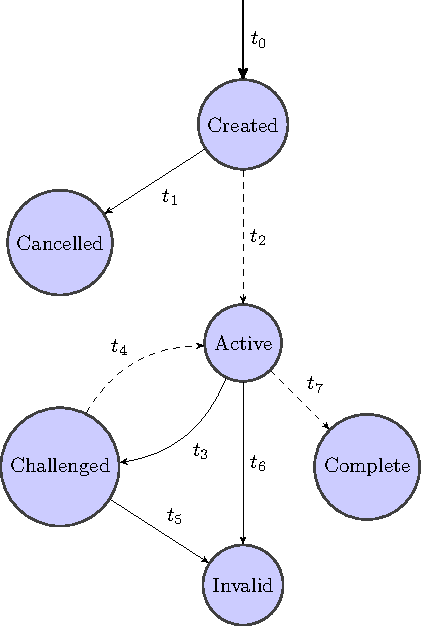
\includegraphics{./contract-state-diagram-figure.pdf}
    \caption{Storage Contract State Diagram}
    \vspace{-0.05in}
\end{figure}

\begin{table}
\centering
\begin{tabular}{|p{1.8cm}|p{1.5cm}|p{8cm}|}
\hline
\textbf{Transition} & \textbf{Actor} & \textbf{Description} \\
\hline
    $t_0$ & Client &
    Creates a new contract. Specifies amount, guarantee, provider,
    deadline. Sets up a server to serve the file.\\
\hline
    $t_1$ & Client  &
    Cancels the contract before the provider activates it.\\
\hline
    $t_2$ & Provider  &
    Receives the file. Proves he owns it and activates the contract. Also,
    has to send the required guarantee.\\
\hline
    $t_3$ & Client  &
    Requests from the provider to prove (on-chain) that he still owns the 
    file.\\
\hline
    $t_4$ & Provider  &
    Proves (on-chain) that he still owns the file.\\
\hline
    $t_5$ & Client  &
    The provider failed to prove that he owns the file (in a given time period).
    Therefore the client can invalidate the contract (receiving the guarantee).\\
\hline
    $t_6$ & Client  &
    The provider failed to prove that he owns the file after the contract
    deadline. Therefore the client can invalidate the contract (receiving the 
    guarantee).\\
\hline
    $t_7$ & Provider  &
    Proves that he still owns the file, during a transition period specified
    in the contract after the deadline. Receives payment.\\
\hline
\end{tabular}
\end{table}

\end{document}
